%!TEX root = Report.tex

\subsection{Graphical user interface}

\todo{Insert screenshot of GUI}

In order to use the system to track ants, we need a user interface. The requirements for the user interface are the following

\begin{itemize}
  \item{It should be able to show the camera feed from both the mobile and the overhead camera}
  \item{It should be able to calibrate the system before initiating the tracking procedure}
  \item{It should provide a way to gather statistics during the process of tracking}
  \item{It should provide a set of controls to manipulate the plotter manually}
\end{itemize}

We chose to implement the GUI in Windows Forms using C\# as Visual Studio provides a convenient way of dragging and dropping of UI controls. Furthermore, it was a requirement that all software would run at least on Windows but preferably on ther platforms as well. We experimented with a Swing GUI in Java, however we experienced some problems with calling into unmanaged C++ code on OSX using Java Native Interface (JNI) so we chose to switch to C\# in order to save time. \\

Furthermore, it is easy to integrate unmanaged code with .NET as no libraries like JNI are needed. All C++ logic is published as a DLL with an interface represented in the GUI code as a list of static methods qualified with the "extern" keyword and called using P/Invoke. The GUI is shown in Fig. \ref{fig:gui}. \\

As seen from the figure, the GUI consists of a horizontal menu bar in the top, a video feed for the mobile camera on the left and a video feed for the overhead camera on the right. In the bottom, a panel is placed to display various statistics about the tracking process and the current performance of the system such as processing time, etc. \\

The GUI provides two modes - one for calibration and one for tracking. Switching between tracking and calibration mode is done through the "Mode" menu point in the top menu. When in calibration mode, the right camera feed will switch and show a threshold of the mobile view instead. Likewise, the lower panel will reveal a slider for setting the thresholdvalue. Thresholding is one of the key techniques behind the tracking and varies with the light and general surroundings of the camera, so it is important to be able to adjust it between sessions. The result of changing the thresholdvalue is visible in real time in the right camera feed and also during tracking if needed. Thus, it is possible to stay in calibration mode while tracking. \\

Ideally, the camera should be located above the ant when setting the thresholdvalue, as we are essentially telling the system how to identify the ant. To do this, open the manual steering panel by selecting "manual steering" from the plotter menu in the top bar. This panel provides controls similar to the arrow keys on a keyboard for manipulating the plotter. Using the keys and the camera feeds and provided that the ant is not moving too quickly, it is possible to adjust the plotter so the camera is located above the ant. Note: this process might require leaving the ant in the freezer for a couple of minutes beforehand. By default, the plotter will move 5 units each time a button is chosen. This number can be adjusted for each axis individually by setting the text fields in the right side of the window. Alternatively, use the controls in the top of the window to go directly to a specific coordinate. \\

When the camera is in place, return to the slider and adjust it until the ant is the largest white blob on screen. Ideally, the ant should be the only white object, but the system will look for the largest object so a reasonable amount of minor objects or "dust" are allowed to be visible as well. \\

When thresholding is in place, tracking is started by choosing "Start" under "Tracking" in the top menu. The camera will track the ant and show statistics in the panel until the user presses "Stop" or the ant is lost in the picture. In either case, the process can be repeated to start tracking again.

%What was the reqs for the GUI?
%How did we want it to look?
%What tasks do we expect the users to do (normal work flow)?
%Are we satisfied with the GUI (eval)?
%JNI skulle være cross platform men fungerede ikke med OpenCV.
%(nævn at det ville have været nice at have det cross platform)
%Vi har ikke noget der finder myren til at starte med. Hvordan kunne dette gøres?

\begin{figure}[!ht]
    \centering
    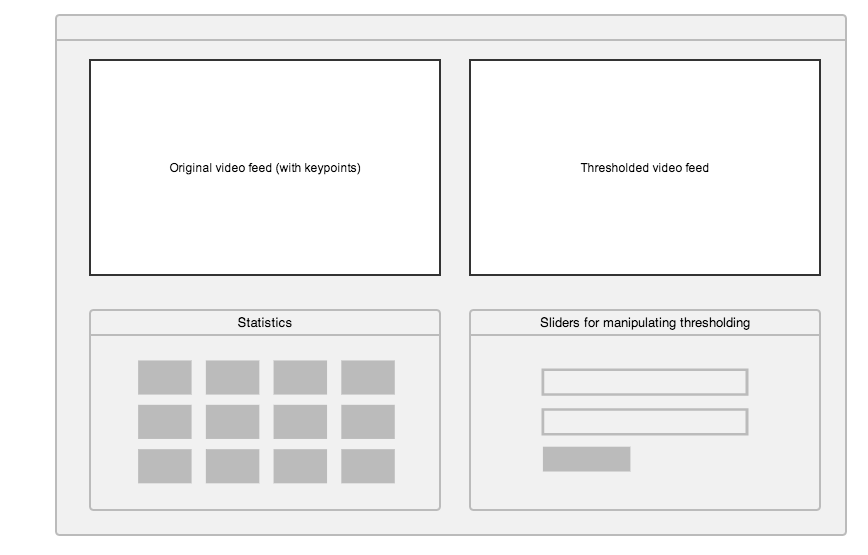
\includegraphics[scale = 0.3]{img/termes_gui.png}
    \caption{Initial GUI draft}
    \label{fig:gui}
\end{figure}

\subsubsection{Statistics} \mbox{}\par
%What statistics do we extract?
%How do the users do this?
%How are they produced?
%Can they be improved (future work)?

TODO
